% !TeX program = pdflatex
% Compilare con: pdflatex Relazione.tex  (due volte, per riferimenti e indice)
\documentclass[11pt,a4paper]{article}

\usepackage[utf8]{inputenc}
\usepackage[T1]{fontenc}
\usepackage[italian]{babel}
\usepackage{lmodern}
\usepackage{amsmath,amssymb}
\usepackage{booktabs}
\usepackage{array}
\usepackage{graphicx}
\usepackage{caption}
\usepackage{geometry}
\usepackage{xcolor}
\usepackage{listings}
\usepackage{enumitem}
\usepackage[hidelinks]{hyperref}

\geometry{margin=2.5cm}

% ------------------------------------------------------------------
% Stile per i blocchi di codice / pseudocodice
% ------------------------------------------------------------------
\definecolor{codebg}{rgb}{0.97,0.97,0.97}
\definecolor{codekw}{rgb}{0.10,0.30,0.65}
\definecolor{codecm}{rgb}{0.35,0.55,0.35}
\definecolor{codest}{rgb}{0.55,0.10,0.55}
\definecolor{codenum}{rgb}{0.45,0.45,0.45}
\lstset{
  basicstyle=\ttfamily\small,
  backgroundcolor=\color{codebg},
  keywordstyle=\color{codekw}\bfseries,
  commentstyle=\color{codecm}\itshape,
  stringstyle=\color{codest},
  numberstyle=\ttfamily\footnotesize\color{codenum},
  showstringspaces=false,
  breaklines=true,
  frame=single,
  framerule=0pt,
  rulecolor=\color{codebg},
  xleftmargin=10pt,
  xrightmargin=8pt,
  aboveskip=8pt,
  belowskip=8pt,
  literate=%
    {à}{{\`a}}1 {è}{{\`e}}1 {é}{{\'e}}1 {ì}{{\`i}}1 {ò}{{\`o}}1 {ù}{{\`u}}1
    {⁻}{{$^{-}$}}1 {·}{{$\cdot$}}1
}
\lstdefinestyle{py}{language=Python}
% Stile per i listati dell'appendice: numeri di riga a sinistra
\lstdefinestyle{pyfull}{language=Python,numbers=left,numbersep=8pt}

% comando per intestazioni di colonna allineate a destra
\newcolumntype{R}{>{\raggedleft\arraybackslash}p{1.7cm}}

\begin{document}

% ==================================================================
% Frontespizio in stile dipartimento
% ==================================================================
\begin{titlepage}
\centering
\vspace*{2cm}

{\large Università degli Studi di Milano Bicocca\par}
{\large Scuola di Scienze\par}
{\large Dipartimento di Informatica, Sistemistica e Comunicazione\par}
\vspace{0.8cm}
{\large Metodi del Calcolo Scientifico\par}

\vspace{2.2cm}
{\Huge\bfseries Progetto 1\par}
\vspace{0.6cm}
{\Large Solutori iterativi per sistemi lineari simmetrici e definiti positivi\par}

\vspace{2.2cm}
\rule{0.55\textwidth}{0.4pt}\par
\vspace{0.6cm}
{\large\bfseries Relazione\par}
\vspace{0.6cm}

\vspace{1.6cm}
{\large Matias Bonoli\par}

\vfill
{\large Anno Accademico 2025--2026\par}
\vspace{0.3cm}
{\large 24 giugno 2026\par}
\end{titlepage}

\tableofcontents
\newpage

% ==================================================================
\section{Introduzione}
% ==================================================================
L'obiettivo principale di questo progetto è lo studio e l'implementazione pratica
dei principali \emph{metodi iterativi} per la risoluzione di sistemi lineari
$A\mathbf{x}=\mathbf{b}$, nel caso in cui la matrice $A$ sia simmetrica e definita
positiva (SPD). Il lavoro che abbiamo svolto si articola in due fasi principali.

Nella prima parte abbiamo curato l'inquadramento algoritmico dei quattro metodi
richiesti dalla traccia --- Jacobi, Gauss--Seidel, Gradiente e Gradiente
coniugato --- partendo dalla loro derivazione teorica (lo \emph{splitting}
$A=P-N$ per i metodi stazionari e l'interpretazione come problema di minimo per i
metodi del gradiente) e fissando il criterio di arresto e la procedura di
validazione comune a tutti.

Nella seconda parte abbiamo sviluppato una piccola \emph{libreria} che implementa
concretamente questi algoritmi. Abbiamo scelto un'architettura coesa, in cui lo
scheletro di iterazione è scritto una sola volta e ogni metodo fornisce soltanto
la propria regola di aggiornamento, e abbiamo dotato il progetto di un eseguibile
da riga di comando che, su un insieme di matrici reali, misura per ciascun metodo
il numero di iterazioni, l'errore di ricostruzione e i tempi di calcolo al
variare della tolleranza richiesta.

\subsection{Linguaggio e dipendenze}
Il progetto è interamente scritto in \textbf{Python 3.12}. Tutti i pacchetti
utilizzati sono \emph{open source}:
\begin{itemize}[leftmargin=1.6em]
  \item \texttt{numpy}: gestione di array e operazioni vettoriali (prodotto
  scalare, norma euclidea, aggiornamenti elemento per elemento);
  \item \texttt{scipy.sparse}: struttura dati per la matrice in formato sparso
  CSR e prodotto matrice--vettore $A\mathbf{v}$;
  \item \texttt{scipy.io.mmread}: lettura dei file in formato MatrixMarket
  \texttt{.mtx};
  \item \texttt{numba}: compilazione JIT della sola \emph{sweep} di
  Gauss--Seidel (intrinsecamente sequenziale), per renderla veloce restando
  codice nostro;
  \item \texttt{matplotlib}: generazione dei grafici di sintesi;
  \item \texttt{scipy.sparse.linalg.eigsh}: usato \emph{solo} nello script di
  analisi a margine, per stimare gli autovalori estremi e quindi
  $\mathrm{cond}(A)$ ai fini dei commenti (non fa parte dei solutori).
\end{itemize}

È importante sottolineare che, come consentito esplicitamente dalla consegna,
\texttt{scipy}/\texttt{numpy} sono usati \textbf{esclusivamente} per le strutture
dati e le operazioni elementari: \textbf{gli algoritmi risolutivi sono
interamente sviluppati nel progetto}. Non viene usato alcun solutore di sistemi
lineari di libreria (niente \texttt{spsolve}, \texttt{cg},
\texttt{numpy.linalg.solve} e simili).

% ==================================================================
\section{PARTE 1}
% ==================================================================

\subsection{I quattro metodi e il criterio di arresto}
Tutti i metodi che abbiamo implementato assumono $A$ \textbf{SPD}
($A=A^{\mathsf{T}}$ e $\mathbf{v}^{\mathsf{T}}A\mathbf{v}>0$ per ogni
$\mathbf{v}\neq\mathbf{0}$) e partono dallo stesso vettore iniziale nullo
$\mathbf{x}^{(0)}=\mathbf{0}$. Indichiamo con
\[
  \mathbf{r}^{(k)}=\mathbf{b}-A\mathbf{x}^{(k)}
\]
il residuo alla generica iterazione $k$. Il criterio di arresto, comune a tutti i
metodi e richiesto dalla traccia, è formulato sul \textbf{residuo scalato}:
\[
  \frac{\lVert\mathbf{b}-A\mathbf{x}^{(k)}\rVert}{\lVert\mathbf{b}\rVert}
  < \texttt{tol}.
\]
A protezione dei casi di non convergenza, l'iterazione si arresta comunque al
superamento di un numero massimo di passi $\texttt{max\_iter}=20000$, segnalando
in tal caso $\texttt{converged}=\text{False}$.

\subsection{Metodi stazionari: lo splitting \texorpdfstring{$A=P-N$}{A=P-N}}
L'idea alla base dei metodi stazionari è spezzare $A=P-N$ con $P$ facile da
invertire; il sistema diventa l'iterazione di punto fisso
\[
  \mathbf{x}^{(k+1)} = \mathbf{x}^{(k)} + P^{-1}\mathbf{r}^{(k)} .
\]
Un principio centrale che governa la convergenza è il seguente: il metodo
converge per ogni $\mathbf{x}^{(0)}$ \emph{se e solo se} il raggio spettrale
della \emph{matrice di iterazione} $B=P^{-1}N$ soddisfa $\rho(B)<1$. Quanto più
piccolo è $\rho(B)$, tanto più rapidamente l'errore viene abbattuto.

\begin{itemize}[leftmargin=1.6em]
  \item \textbf{Jacobi}: scegliamo $P=D$ (la diagonale di $A$). L'inversa
  $D^{-1}$ è banale (i reciproci degli elementi diagonali), quindi il passo è
  completamente vettoriale e parallelizzabile. La sola ipotesi SPD \emph{non}
  garantisce $\rho(B)<1$ (una condizione sufficiente è che anche $2D-A$ sia SPD,
  oppure la dominanza diagonale di $A$).
  \item \textbf{Gauss--Seidel}: scegliamo $P=D+L$ (la parte triangolare
  inferiore di $A$). Riusando immediatamente le componenti appena aggiornate, di
  norma servono \emph{circa la metà} delle iterazioni di Jacobi. Inoltre, se $A$
  è SPD, Gauss--Seidel converge \textbf{sempre}. Il prezzo è che il passo è una
  sostituzione in avanti, intrinsecamente sequenziale.
\end{itemize}

\subsection{Metodi del gradiente: risolvere equivale a minimizzare}
Per $A$ SPD, risolvere $A\mathbf{x}=\mathbf{b}$ equivale a minimizzare il
funzionale quadratico
\[
  \varphi(\mathbf{y}) = \tfrac12\,\mathbf{y}^{\mathsf{T}}A\mathbf{y}
                        - \mathbf{b}^{\mathsf{T}}\mathbf{y},
  \qquad
  \nabla\varphi(\mathbf{y}) = A\mathbf{y}-\mathbf{b},
\]
il cui gradiente si annulla esattamente in $A\mathbf{y}=\mathbf{b}$. Proprio
perché $A$ è definita positiva, $\varphi$ è un paraboloide a ``ciotola'' e quel
punto stazionario è un minimo.

\begin{itemize}[leftmargin=1.6em]
  \item \textbf{Gradiente} (\emph{steepest descent}): a ogni passo ci si muove
  nella direzione dell'antigradiente $-\nabla\varphi=\mathbf{r}^{(k)}$, con il
  passo ottimo lungo quella retta
  \[
    \alpha_k = \frac{\mathbf{r}^{(k)}\!\cdot\mathbf{r}^{(k)}}
                    {\mathbf{r}^{(k)}\!\cdot A\mathbf{r}^{(k)}},
    \qquad
    \mathbf{x}^{(k+1)}=\mathbf{x}^{(k)}+\alpha_k\mathbf{r}^{(k)}.
  \]
  Il metodo converge sempre per $A$ SPD, ma sulle matrici mal condizionate la
  direzione di massima discesa non punta verso il fondo della valle: si genera il
  caratteristico \emph{zig-zag} e la velocità degrada con il numero di
  condizionamento $\mathrm{cond}(A)=\lambda_{\max}/\lambda_{\min}$.
  \item \textbf{Gradiente coniugato} (CG): le direzioni di ricerca sono
  $A$-coniugate ($\mathbf{d}_i^{\mathsf{T}}A\mathbf{d}_j=0$ per $i\neq j$). Una
  volta ottimizzata una direzione, le successive non la ``rovinano'': niente
  zig-zag. Per $A$ SPD di dimensione $n$, CG raggiunge la soluzione esatta in
  \textbf{al più $n$ iterazioni}; in pratica ne bastano molte meno e il numero di
  iterazioni scala come $\sqrt{\mathrm{cond}(A)}$.
\end{itemize}

\subsection{Un solo prodotto matrice--vettore per iterazione}
Una scelta implementativa che attraversa tutta la PARTE 2 ma che ha radice
algoritmica è quella di usare \textbf{un solo} prodotto matrice--vettore per
iterazione. Per Gradiente e Gradiente coniugato il residuo successivo non viene
ricalcolato come $\mathbf{b}-A\mathbf{x}^{(k+1)}$ (un secondo matvec), ma ottenuto
per ricorrenza
\[
  \mathbf{r}^{(k+1)} = \mathbf{r}^{(k)} - \alpha_k\, A\mathbf{v},
\]
riusando il prodotto $A\mathbf{v}$ già calcolato per determinare il passo. Su
matrici dense questo dimezza il costo dominante dell'iterazione.

% ==================================================================
\section{PARTE 2}
% ==================================================================

\subsection{L'architettura della libreria}
La libreria che abbiamo sviluppato (file \texttt{solvers.py}) \textbf{non è una
sequenza di funzioni indipendenti}, ma una piccola gerarchia di classi coesa,
costruita su un'osservazione: tutti i metodi condividono lo stesso scheletro e
differiscono \emph{soltanto} nel passo di aggiornamento
$\mathbf{x}^{(k)}\to\mathbf{x}^{(k+1)}$. L'architettura si articola in questi
componenti fondamentali:

\begin{enumerate}[leftmargin=1.8em]
  \item \textbf{Lo scheletro comune.} La classe base astratta
  \texttt{IterativeSolver} implementa \emph{una sola volta} il metodo
  \texttt{solve()}: inizializza $\mathbf{x}^{(0)}=\mathbf{0}$, esegue il ciclo che
  si arresta sul residuo scalato (o al superamento di \texttt{max\_iter}), misura
  il tempo e costruisce il risultato.
  \begin{lstlisting}
x^(0) = 0
finche'  ||b - A x^(k)|| / ||b|| >= tol  e  k < max_iter:
    x^(k+1) = aggiornamento(x^(k))
    k += 1
  \end{lstlisting}

  \item \textbf{Il passo specifico.} L'interfaccia astratta \texttt{\_Iteration}
  incapsula lo stato e il \emph{passo} di un metodo (pattern \emph{template
  method}). Le quattro classi concrete --- \texttt{Jacobi},
  \texttt{GaussSeidel}, \texttt{Gradient}, \texttt{ConjugateGradient} ---
  forniscono unicamente la propria regola di aggiornamento. Aggiungere un quinto
  metodo significa scrivere una sola classe, senza toccare lo scheletro.

  \item \textbf{Il risultato uniforme.} La \texttt{dataclass}
  \texttt{SolverResult} raccoglie in modo omogeneo l'esito di ogni risoluzione:
  soluzione approssimata, iterazioni, tempo, residuo relativo finale e flag di
  convergenza.
\end{enumerate}

Le istanze dei quattro metodi sono raccolte nella tupla \texttt{SOLVERS}, su cui
iterano sia il runner sia i test. Le parti di servizio comuni sono fattorizzate
una sola volta (\texttt{\_validate\_for\_iteration} per controllare che la matrice
sia quadrata e con diagonale non nulla; \texttt{\_safe\_norm} per il calcolo della
norma di $\mathbf{b}$).

\subsection{Note implementative rilevanti}
L'implementazione degli algoritmi è strutturata attorno a quattro accorgimenti:
\begin{itemize}[leftmargin=1.6em]
  \item \textbf{Sparsità preservata.} Nessun metodo fattorizza o modifica $A$: la
  matrice è impiegata solo per prodotti $A\mathbf{v}$, il cui costo è
  proporzionale al numero di non-zeri e non a $n^2$ (nessun \emph{fill-in}).

  \item \textbf{Un solo matvec per iterazione.} Come descritto in PARTE 1, per
  Jacobi, Gradiente e Gradiente coniugato il residuo successivo si ottiene per
  ricorrenza, evitando un prodotto matrice--vettore aggiuntivo.

  \item \textbf{Gauss--Seidel senza inversa, ma veloce.} Il passo
  $P^{-1}\mathbf{r}$ (con $P=D+L$) è realizzato da una \emph{sweep} in place che
  aggiorna $\mathbf{x}^{(k+1)}$ riusando i valori appena calcolati --- equivalente
  a una sostituzione in avanti --- \textbf{senza mai costruire $P^{-1}$}. Essendo
  intrinsecamente sequenziale ($x_i$ dipende da $x_0,\dots,x_{i-1}$), questa sweep
  è compilata con \textbf{numba} (\texttt{\_gauss\_seidel\_sweep}), restando
  codice nostro: così non diventa il collo di bottiglia che sarebbe un ciclo
  Python puro.

  \item \textbf{Tempi equi.} Prima delle misure eseguiamo un \emph{warm-up} che
  forza la compilazione JIT su un problemino $3\times3$, così il tempo riportato
  per Gauss--Seidel non include il costo (una tantum) di compilazione.
\end{itemize}

\subsection{Interfaccia da riga di comando}
Per applicare e mettere a confronto i metodi abbiamo realizzato un eseguibile
(\texttt{run\_assignment.py}). L'utente può lanciare l'intera validazione su tutte
le matrici e tolleranze, oppure restringere il calcolo a una specifica matrice
(\texttt{-{}-matrix}), tolleranza (\texttt{-{}-tol}) o metodo
(\texttt{-{}-method}), parametri tutti ripetibili. Il software produce un CSV
numerico con tutte le metriche e tre grafici di sintesi (iterazioni, errore
relativo e tempo al variare della tolleranza), salvabili in una cartella di
output configurabile.

% ==================================================================
\section{Esperimenti}
% ==================================================================
Per ogni matrice abbiamo seguito la procedura di validazione standard richiesta
dalla traccia: fissata la soluzione esatta nota $\mathbf{x}=[1,1,\dots,1]$, il
termine noto è $\mathbf{b}=A\mathbf{x}$ (cioè il vettore delle somme di riga di
$A$), e i quattro metodi partono da $\mathbf{x}^{(0)}=\mathbf{0}$. Avere a
disposizione la soluzione esatta ci permette di misurare l'\textbf{errore vero}
\[
  \frac{\lVert\mathbf{x}_{\text{calc}}-\mathbf{x}\rVert}{\lVert\mathbf{x}\rVert},
\]
cosa impossibile in un problema reale in cui la soluzione non è nota. Ogni
configurazione è stata ripetuta alle quattro tolleranze
$\texttt{tol}\in\{10^{-4},10^{-6},10^{-8},10^{-10}\}$, con
$\texttt{max\_iter}=20000$.

Le misure di tempo sono state condotte sempre sullo stesso ambiente: Intel Core
i7-1165G7 @ 2.80\,GHz, 16\,GB RAM, Windows 11, Python 3.12 con numpy, scipy e
numba.

\subsection{Le matrici di test}
Le quattro matrici fornite si dividono in due famiglie con caratteristiche
opposte, come riassunto nella Tabella~\ref{tab:matrici}.

\begin{table}[h]
\centering
\caption{Caratteristiche delle matrici di test (autovalori e $\mathrm{cond}(A)$
stimati con \texttt{analyze\_cond.py}).}
\label{tab:matrici}
\begin{tabular}{l r r r r r}
\toprule
Matrice & $n$ & non-zeri & $\lambda_{\min}$ & $\lambda_{\max}$ &
$\mathrm{cond}(A)$ \\
\midrule
spa1 & 1000 & 182\,434    & $4.88\cdot10^{-1}$ & $9.99\cdot10^{2}$ & $2.05\cdot10^{3}$ \\
spa2 & 3000 & 1\,633\,298 & $2.12\cdot10^{0}$  & $3.00\cdot10^{3}$ & $1.41\cdot10^{3}$ \\
vem1 & 1681 & 13\,385     & $1.23\cdot10^{-2}$ & $4.00\cdot10^{0}$ & $3.25\cdot10^{2}$ \\
vem2 & 2601 & 21\,225     & $7.89\cdot10^{-3}$ & $4.00\cdot10^{0}$ & $5.07\cdot10^{2}$ \\
\bottomrule
\end{tabular}
\end{table}

Le \texttt{spa*} sono molto più dense ($\approx$180 e $\approx$540 non-zeri per
riga) e con condizionamento maggiore; le \texttt{vem*} sono molto più sparse
($\approx$8 non-zeri per riga) e meglio condizionate. Come vedremo, questa
differenza strutturale si riflette in modo netto sulle prestazioni dei diversi
metodi.

\subsection{Risultati numerici}
Le tabelle seguenti riportano i risultati completi estratti da
\texttt{results/results.csv}. Tutti i metodi sono arrivati a convergenza
($\text{conv}=\text{sì}$) entro $\texttt{max\_iter}=20000$. I tempi sono in
secondi sull'ambiente indicato (soggetti a variazioni di runtime fra esecuzioni).

\begin{table}[h]
\centering
\caption{\texttt{spa1} --- $n=1000$, nnz $=182\,434$.}
\begin{tabular}{l l r r r r}
\toprule
tol & metodo & iter & err.\ rel. & res.\ scal. & $t$ [s] \\
\midrule
$10^{-4}$  & Jacobi              & 115   & $1.77\cdot10^{-3}$ & $9.48\cdot10^{-5}$ & 0.080 \\
$10^{-4}$  & Gauss--Seidel       & 9     & $1.82\cdot10^{-2}$ & $7.79\cdot10^{-5}$ & 0.017 \\
$10^{-4}$  & Gradiente           & 143   & $3.46\cdot10^{-2}$ & $9.91\cdot10^{-5}$ & 0.093 \\
$10^{-4}$  & Gradiente coniugato & 49    & $2.08\cdot10^{-2}$ & $9.78\cdot10^{-5}$ & 0.031 \\
\midrule
$10^{-6}$  & Jacobi              & 181   & $1.80\cdot10^{-5}$ & $9.62\cdot10^{-7}$ & 0.110 \\
$10^{-6}$  & Gauss--Seidel       & 17    & $1.30\cdot10^{-4}$ & $5.58\cdot10^{-7}$ & 0.031 \\
$10^{-6}$  & Gradiente           & 3577  & $9.68\cdot10^{-4}$ & $9.98\cdot10^{-7}$ & 2.172 \\
$10^{-6}$  & Gradiente coniugato & 134   & $2.55\cdot10^{-5}$ & $9.74\cdot10^{-7}$ & 0.091 \\
\midrule
$10^{-8}$  & Jacobi              & 247   & $1.82\cdot10^{-7}$ & $9.76\cdot10^{-9}$ & 0.168 \\
$10^{-8}$  & Gauss--Seidel       & 24    & $1.71\cdot10^{-6}$ & $7.34\cdot10^{-9}$ & 0.038 \\
$10^{-8}$  & Gradiente           & 8233  & $9.82\cdot10^{-6}$ & $9.99\cdot10^{-9}$ & 5.819 \\
$10^{-8}$  & Gradiente coniugato & 177   & $1.32\cdot10^{-7}$ & $9.03\cdot10^{-9}$ & 0.140 \\
\midrule
$10^{-10}$ & Jacobi              & 313   & $1.85\cdot10^{-9}$  & $9.91\cdot10^{-11}$ & 0.241 \\
$10^{-10}$ & Gauss--Seidel       & 31    & $2.25\cdot10^{-8}$  & $9.65\cdot10^{-11}$ & 0.058 \\
$10^{-10}$ & Gradiente           & 12919 & $9.82\cdot10^{-8}$  & $9.99\cdot10^{-11}$ & 10.171 \\
$10^{-10}$ & Gradiente coniugato & 200   & $1.20\cdot10^{-9}$  & $7.94\cdot10^{-11}$ & 0.156 \\
\bottomrule
\end{tabular}
\end{table}

\begin{table}[h]
\centering
\caption{\texttt{spa2} --- $n=3000$, nnz $=1\,633\,298$.}
\begin{tabular}{l l r r r r}
\toprule
tol & metodo & iter & err.\ rel. & res.\ scal. & $t$ [s] \\
\midrule
$10^{-4}$  & Jacobi              & 36   & $1.77\cdot10^{-3}$ & $9.54\cdot10^{-5}$ & 0.259 \\
$10^{-4}$  & Gauss--Seidel       & 5    & $2.60\cdot10^{-3}$ & $4.14\cdot10^{-5}$ & 0.088 \\
$10^{-4}$  & Gradiente           & 161  & $1.81\cdot10^{-2}$ & $9.90\cdot10^{-5}$ & 1.176 \\
$10^{-4}$  & Gradiente coniugato & 42   & $9.82\cdot10^{-3}$ & $9.91\cdot10^{-5}$ & 0.306 \\
\midrule
$10^{-6}$  & Jacobi              & 57   & $1.67\cdot10^{-5}$ & $9.00\cdot10^{-7}$ & 0.419 \\
$10^{-6}$  & Gauss--Seidel       & 8    & $5.14\cdot10^{-5}$ & $7.85\cdot10^{-7}$ & 0.146 \\
$10^{-6}$  & Gradiente           & 1949 & $6.69\cdot10^{-4}$ & $9.99\cdot10^{-7}$ & 12.249 \\
$10^{-6}$  & Gradiente coniugato & 122  & $1.20\cdot10^{-4}$ & $9.09\cdot10^{-7}$ & 0.692 \\
\midrule
$10^{-8}$  & Jacobi              & 78   & $1.57\cdot10^{-7}$ & $8.49\cdot10^{-9}$ & 0.480 \\
$10^{-8}$  & Gauss--Seidel       & 12   & $2.79\cdot10^{-7}$ & $4.27\cdot10^{-9}$ & 0.178 \\
$10^{-8}$  & Gradiente           & 5087 & $6.87\cdot10^{-6}$ & $9.98\cdot10^{-9}$ & 34.083 \\
$10^{-8}$  & Gradiente coniugato & 196  & $5.59\cdot10^{-7}$ & $9.60\cdot10^{-9}$ & 1.387 \\
\midrule
$10^{-10}$ & Jacobi              & 99   & $1.48\cdot10^{-9}$ & $8.01\cdot10^{-11}$ & 0.706 \\
$10^{-10}$ & Gauss--Seidel       & 15   & $5.57\cdot10^{-9}$ & $8.52\cdot10^{-11}$ & 0.262 \\
$10^{-10}$ & Gradiente           & 8285 & $6.94\cdot10^{-8}$ & $9.99\cdot10^{-11}$ & 58.376 \\
$10^{-10}$ & Gradiente coniugato & 240  & $5.32\cdot10^{-9}$ & $9.82\cdot10^{-11}$ & 1.613 \\
\bottomrule
\end{tabular}
\end{table}

\begin{table}[h]
\centering
\caption{\texttt{vem1} --- $n=1681$, nnz $=13\,385$.}
\begin{tabular}{l l r r r r}
\toprule
tol & metodo & iter & err.\ rel. & res.\ scal. & $t$ [s] \\
\midrule
$10^{-4}$  & Jacobi              & 1314 & $3.54\cdot10^{-3}$ & $9.99\cdot10^{-5}$ & 0.084 \\
$10^{-4}$  & Gauss--Seidel       & 659  & $3.51\cdot10^{-3}$ & $9.93\cdot10^{-5}$ & 0.136 \\
$10^{-4}$  & Gradiente           & 890  & $2.70\cdot10^{-3}$ & $9.93\cdot10^{-5}$ & 0.098 \\
$10^{-4}$  & Gradiente coniugato & 38   & $4.08\cdot10^{-5}$ & $7.11\cdot10^{-5}$ & 0.003 \\
\midrule
$10^{-6}$  & Jacobi              & 2433 & $3.54\cdot10^{-5}$ & $9.99\cdot10^{-7}$ & 0.219 \\
$10^{-6}$  & Gauss--Seidel       & 1218 & $3.53\cdot10^{-5}$ & $9.99\cdot10^{-7}$ & 0.197 \\
$10^{-6}$  & Gradiente           & 1612 & $2.71\cdot10^{-5}$ & $9.97\cdot10^{-7}$ & 0.155 \\
$10^{-6}$  & Gradiente coniugato & 45   & $3.73\cdot10^{-7}$ & $8.90\cdot10^{-7}$ & 0.004 \\
\midrule
$10^{-8}$  & Jacobi              & 3552 & $3.54\cdot10^{-7}$ & $9.99\cdot10^{-9}$ & 0.273 \\
$10^{-8}$  & Gauss--Seidel       & 1778 & $3.52\cdot10^{-7}$ & $9.96\cdot10^{-9}$ & 0.328 \\
$10^{-8}$  & Gradiente           & 2336 & $2.70\cdot10^{-7}$ & $9.90\cdot10^{-9}$ & 0.231 \\
$10^{-8}$  & Gradiente coniugato & 53   & $2.83\cdot10^{-9}$ & $7.80\cdot10^{-9}$ & 0.005 \\
\midrule
$10^{-10}$ & Jacobi              & 4671 & $3.54\cdot10^{-9}$  & $9.99\cdot10^{-11}$ & 0.352 \\
$10^{-10}$ & Gauss--Seidel       & 2338 & $3.51\cdot10^{-9}$  & $9.94\cdot10^{-11}$ & 0.370 \\
$10^{-10}$ & Gradiente           & 3058 & $2.71\cdot10^{-9}$  & $9.97\cdot10^{-11}$ & 0.297 \\
$10^{-10}$ & Gradiente coniugato & 59   & $2.19\cdot10^{-11}$ & $6.91\cdot10^{-11}$ & 0.005 \\
\bottomrule
\end{tabular}
\end{table}

\begin{table}[h]
\centering
\caption{\texttt{vem2} --- $n=2601$, nnz $=21\,225$.}
\begin{tabular}{l l r r r r}
\toprule
tol & metodo & iter & err.\ rel. & res.\ scal. & $t$ [s] \\
\midrule
$10^{-4}$  & Jacobi              & 1927 & $4.97\cdot10^{-3}$ & $9.99\cdot10^{-5}$ & 0.198 \\
$10^{-4}$  & Gauss--Seidel       & 965  & $4.95\cdot10^{-3}$ & $9.98\cdot10^{-5}$ & 0.223 \\
$10^{-4}$  & Gradiente           & 1308 & $3.81\cdot10^{-3}$ & $9.98\cdot10^{-5}$ & 0.159 \\
$10^{-4}$  & Gradiente coniugato & 47   & $5.73\cdot10^{-5}$ & $9.19\cdot10^{-5}$ & 0.006 \\
\midrule
$10^{-6}$  & Jacobi              & 3676 & $4.97\cdot10^{-5}$ & $9.99\cdot10^{-7}$ & 0.381 \\
$10^{-6}$  & Gauss--Seidel       & 1840 & $4.94\cdot10^{-5}$ & $9.96\cdot10^{-7}$ & 0.557 \\
$10^{-6}$  & Gradiente           & 2438 & $3.79\cdot10^{-5}$ & $9.92\cdot10^{-7}$ & 0.321 \\
$10^{-6}$  & Gradiente coniugato & 56   & $4.74\cdot10^{-7}$ & $8.54\cdot10^{-7}$ & 0.009 \\
\midrule
$10^{-8}$  & Jacobi              & 5425 & $4.97\cdot10^{-7}$ & $9.99\cdot10^{-9}$ & 0.738 \\
$10^{-8}$  & Gauss--Seidel       & 2714 & $4.96\cdot10^{-7}$ & $9.99\cdot10^{-9}$ & 0.720 \\
$10^{-8}$  & Gradiente           & 3566 & $3.81\cdot10^{-7}$ & $9.97\cdot10^{-9}$ & 0.588 \\
$10^{-8}$  & Gradiente coniugato & 66   & $4.30\cdot10^{-9}$ & $8.60\cdot10^{-9}$ & 0.011 \\
\midrule
$10^{-10}$ & Jacobi              & 7174 & $4.96\cdot10^{-9}$  & $9.98\cdot10^{-11}$ & 0.819 \\
$10^{-10}$ & Gauss--Seidel       & 3589 & $4.95\cdot10^{-9}$  & $9.97\cdot10^{-11}$ & 0.230 \\
$10^{-10}$ & Gradiente           & 4696 & $3.80\cdot10^{-9}$  & $9.94\cdot10^{-11}$ & 0.157 \\
$10^{-10}$ & Gradiente coniugato & 74   & $2.25\cdot10^{-11}$ & $5.90\cdot10^{-11}$ & 0.002 \\
\bottomrule
\end{tabular}
\end{table}

\clearpage
\subsection{Grafici di sintesi}
\begin{figure}[h]
\centering
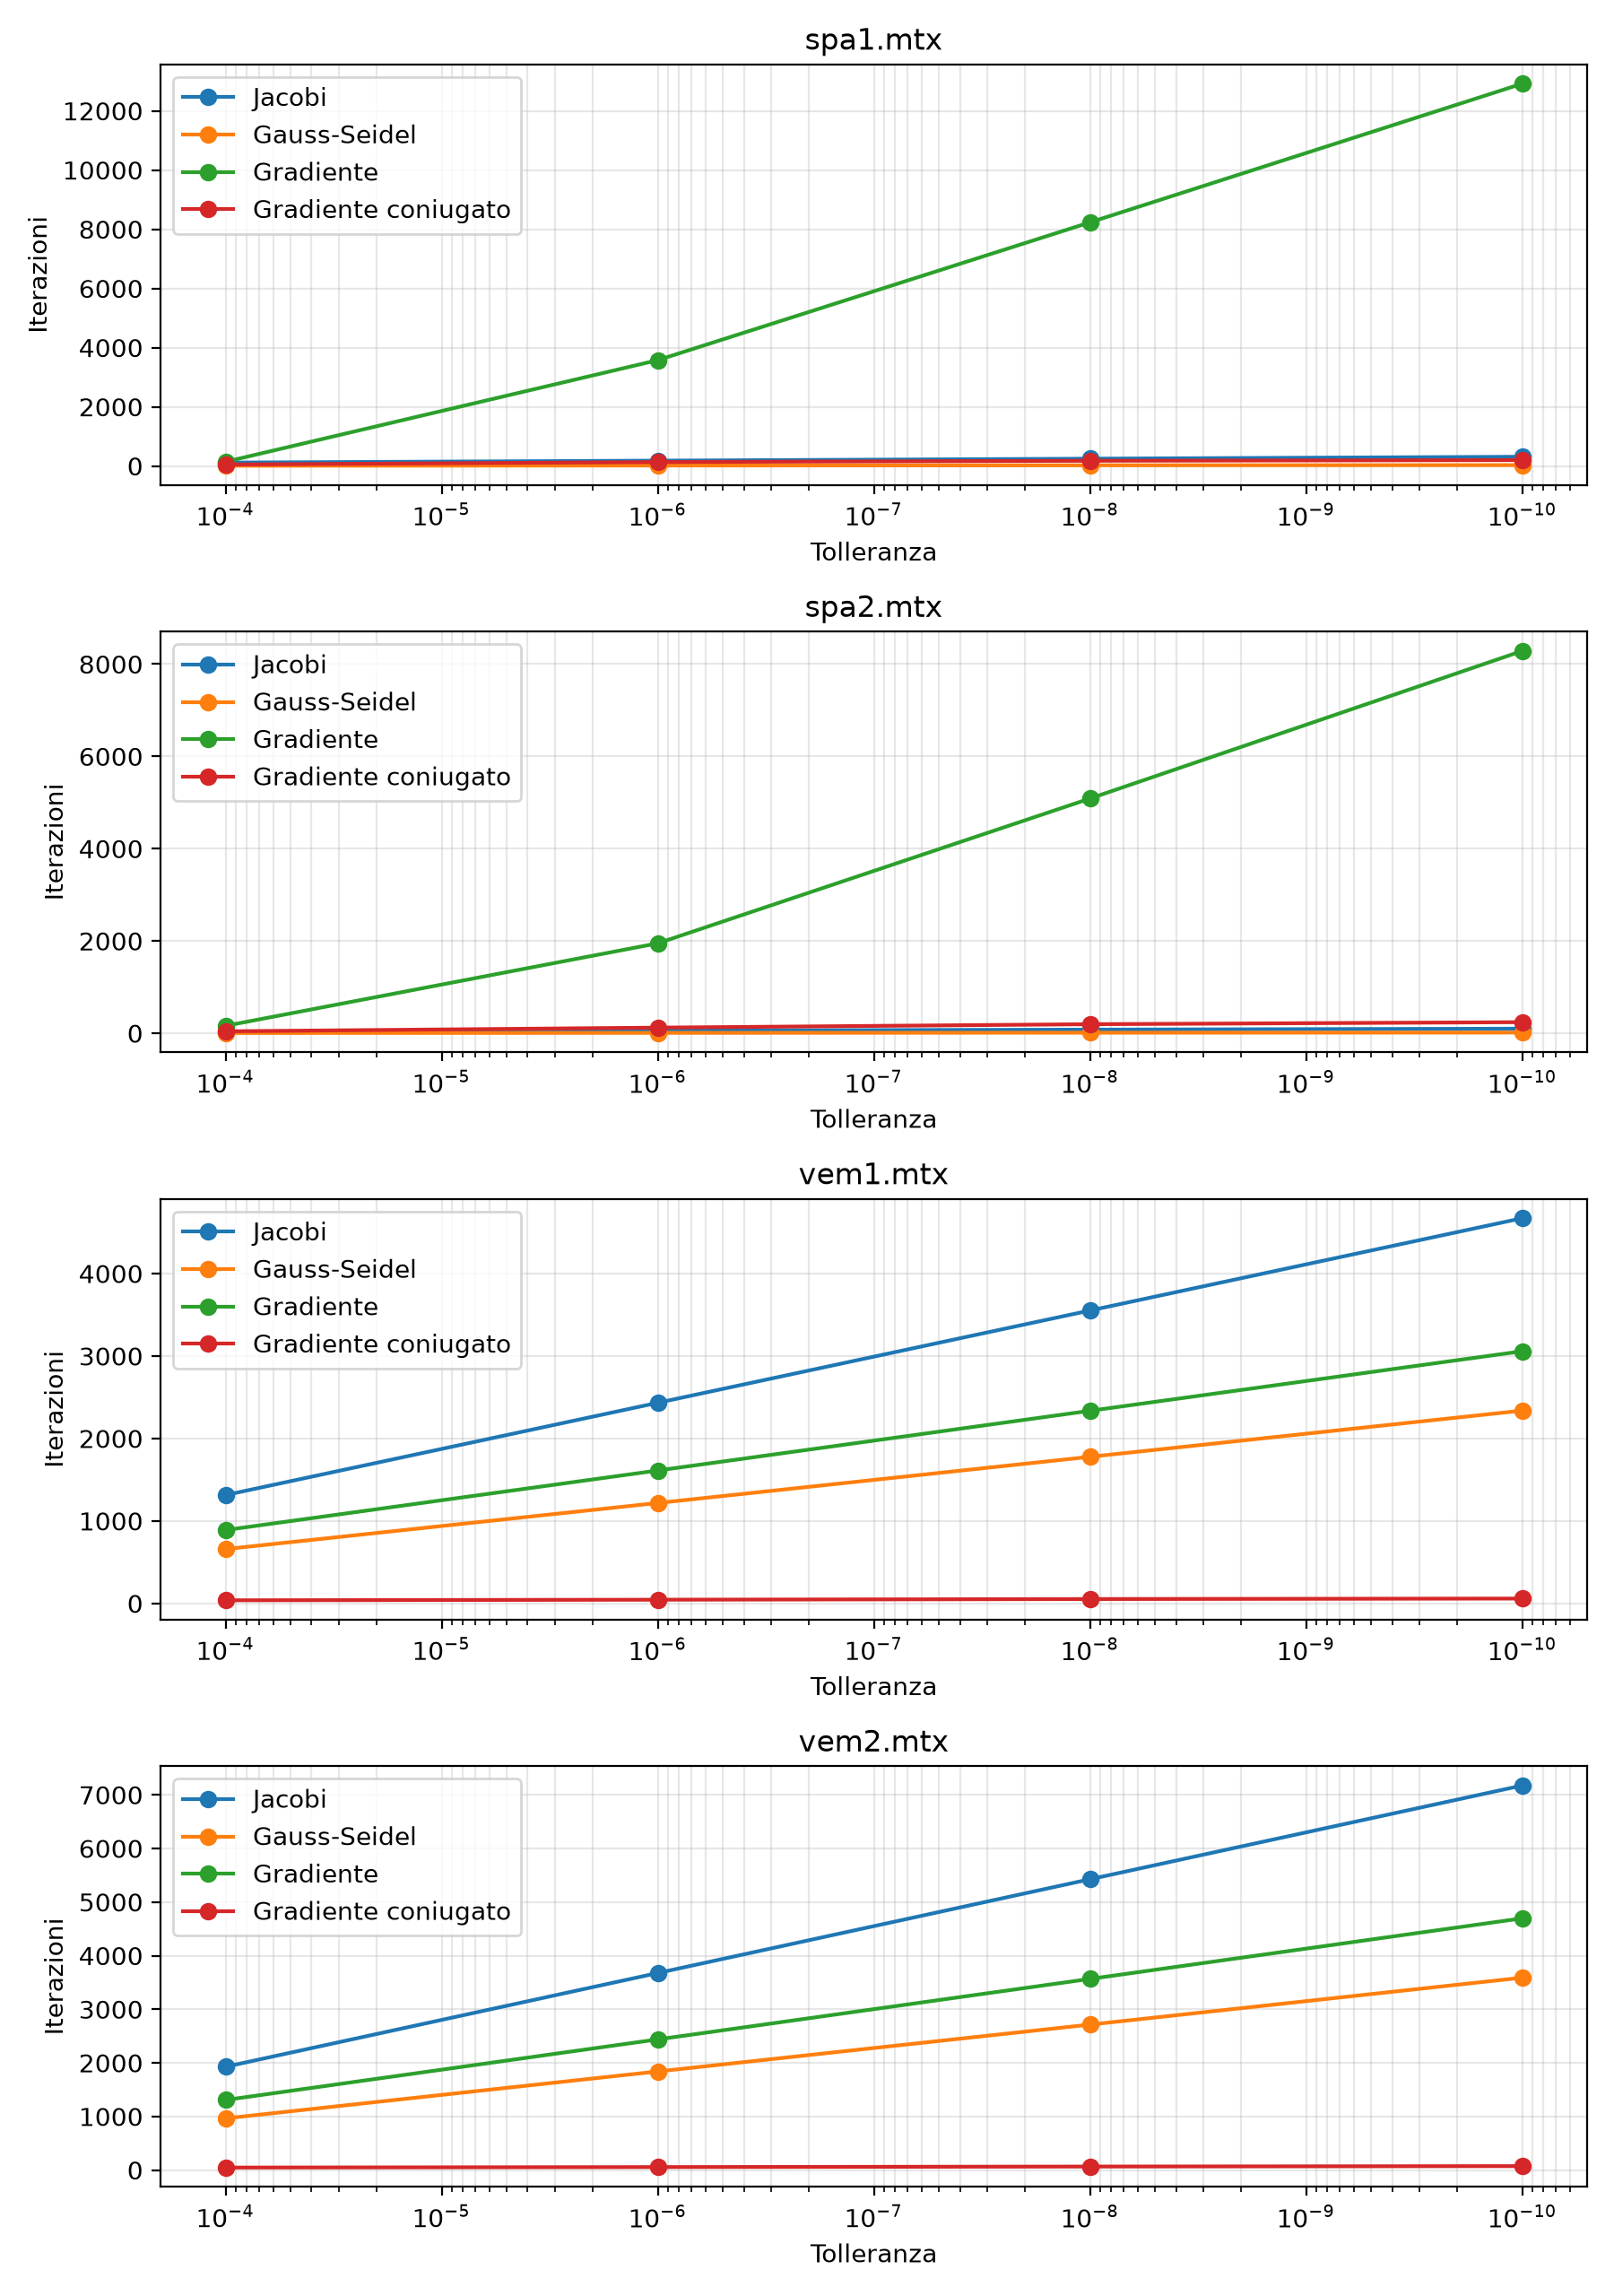
\includegraphics[width=0.85\textwidth]{results/plots/iterations.png}
\caption{Numero di iterazioni al variare di \texttt{tol} (asse $x$ in scala
logaritmica, una riga per matrice).}
\end{figure}

\begin{figure}[h]
\centering
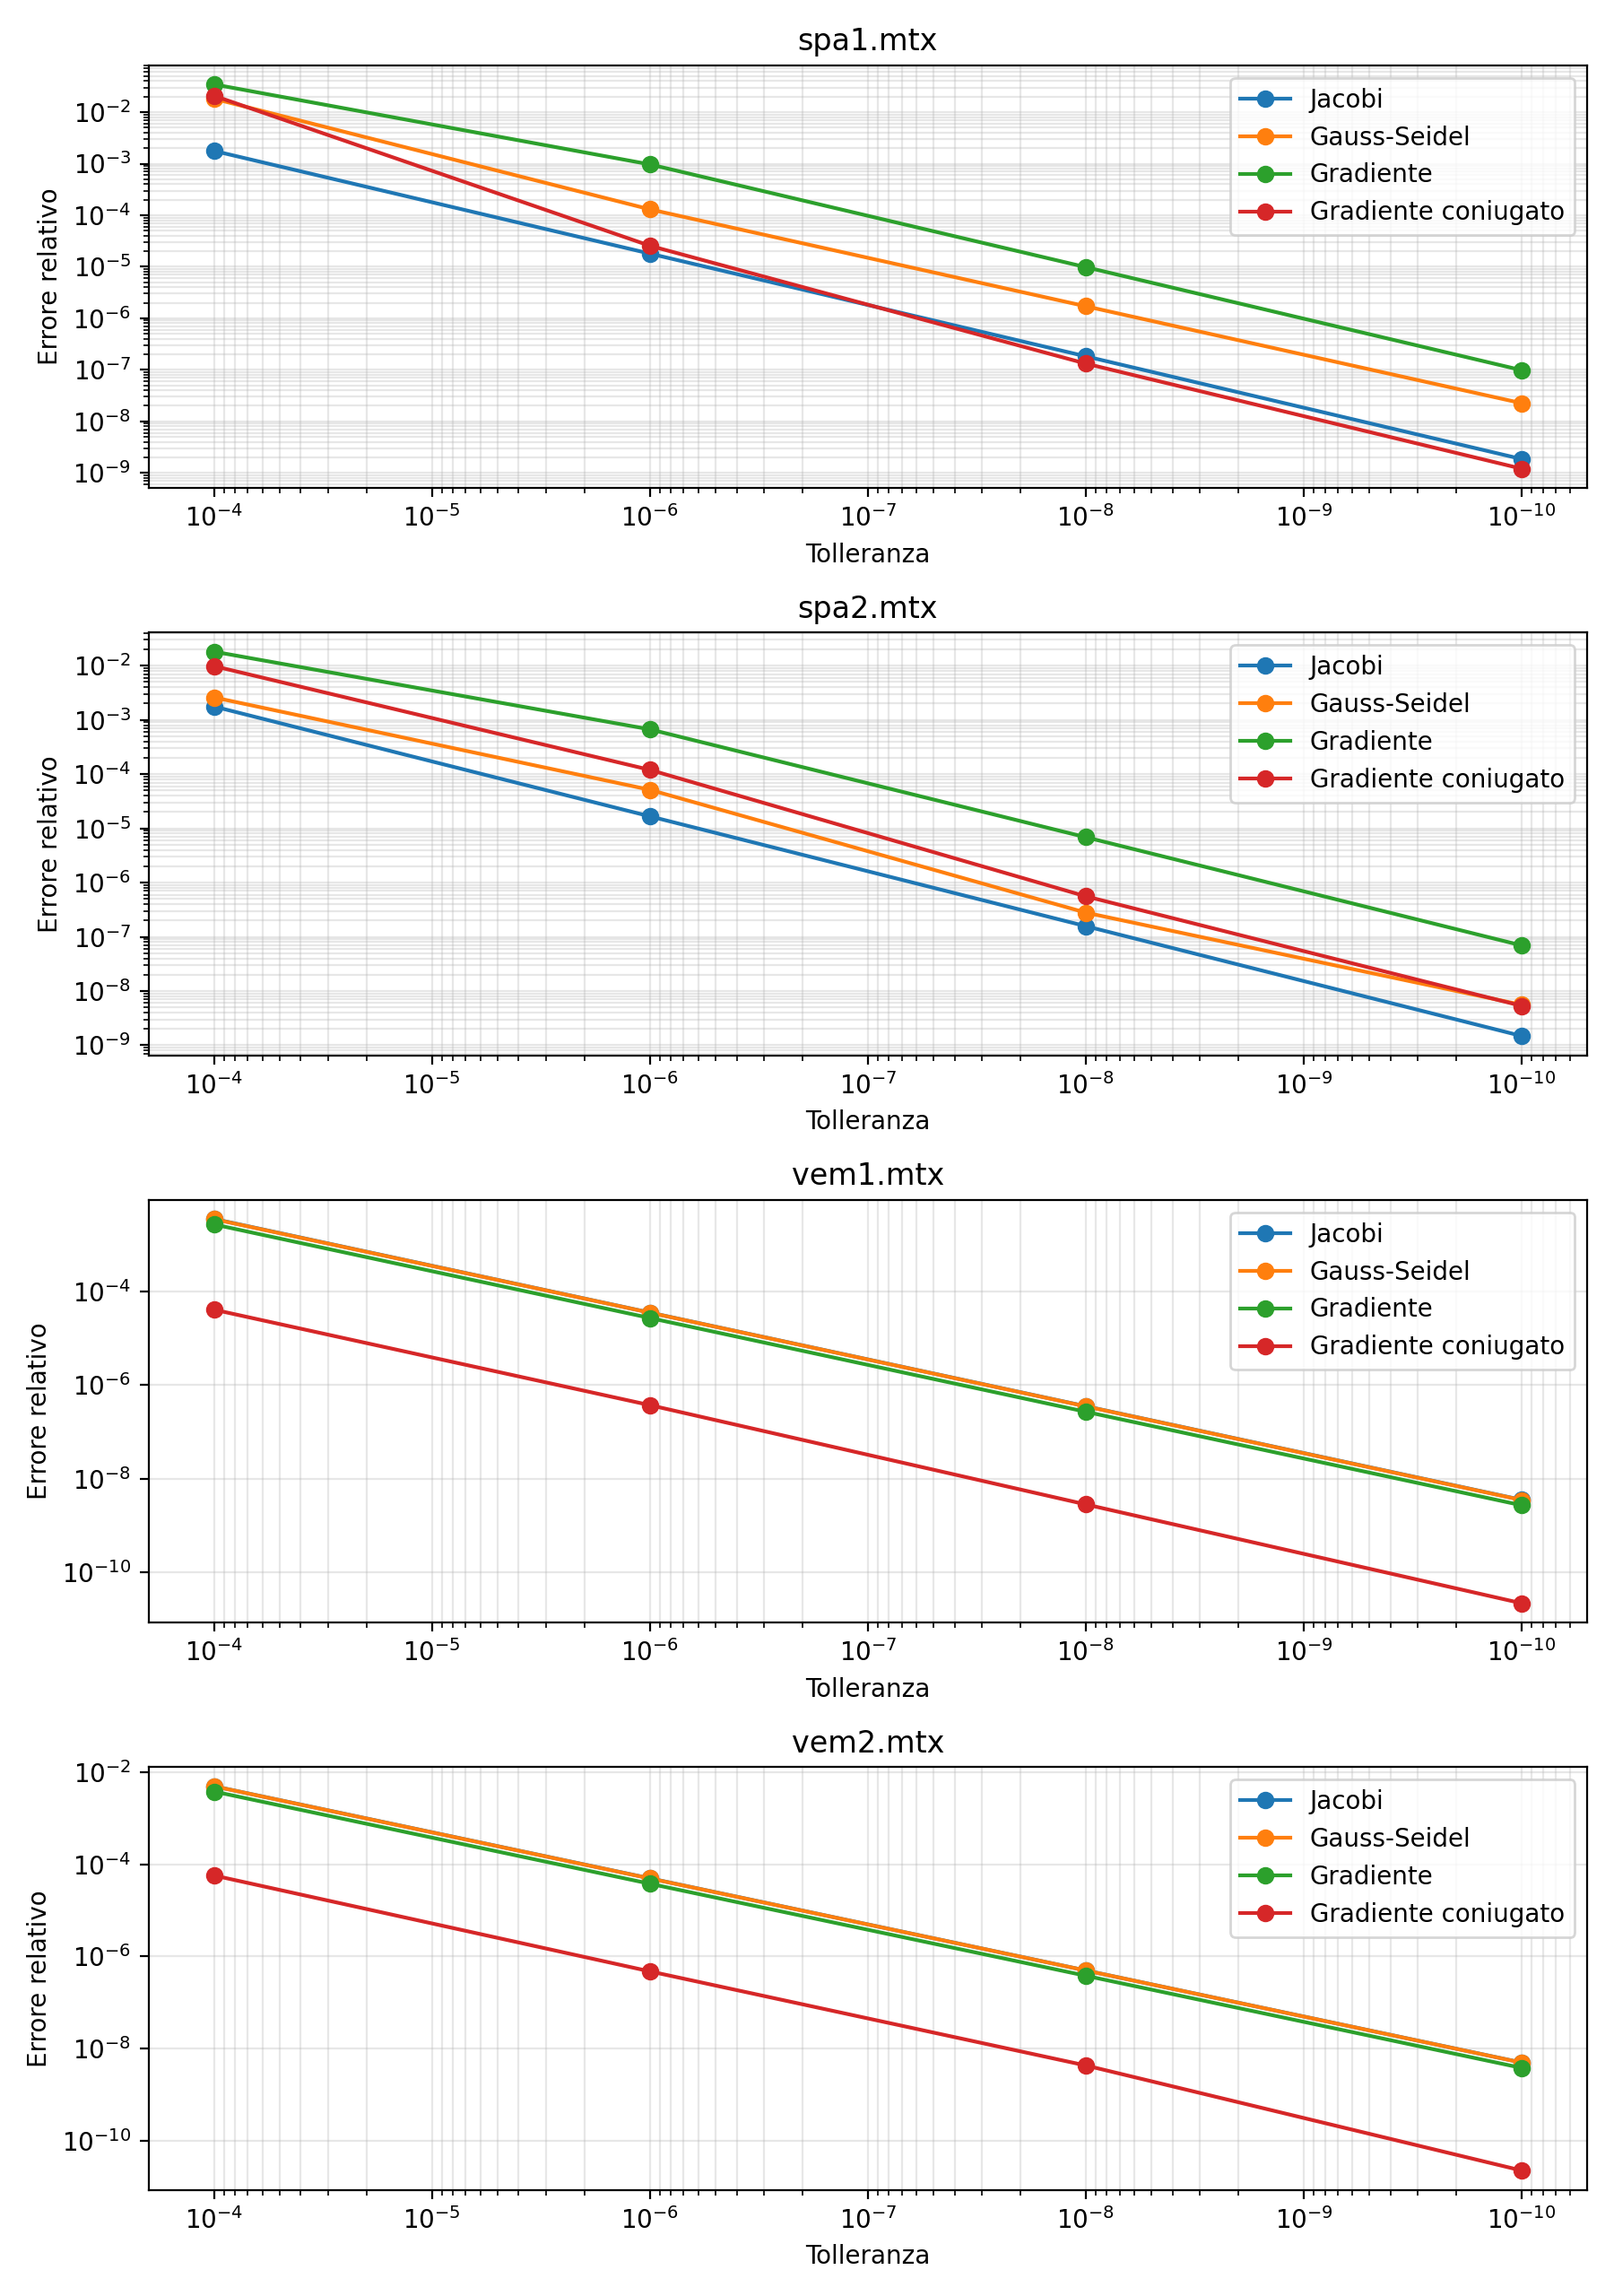
\includegraphics[width=0.85\textwidth]{results/plots/relative_error.png}
\caption{Errore relativo $\lVert\mathbf{x}_{\text{calc}}-\mathbf{x}\rVert/
\lVert\mathbf{x}\rVert$ al variare di \texttt{tol} (scala logaritmica).}
\end{figure}

\begin{figure}[h]
\centering
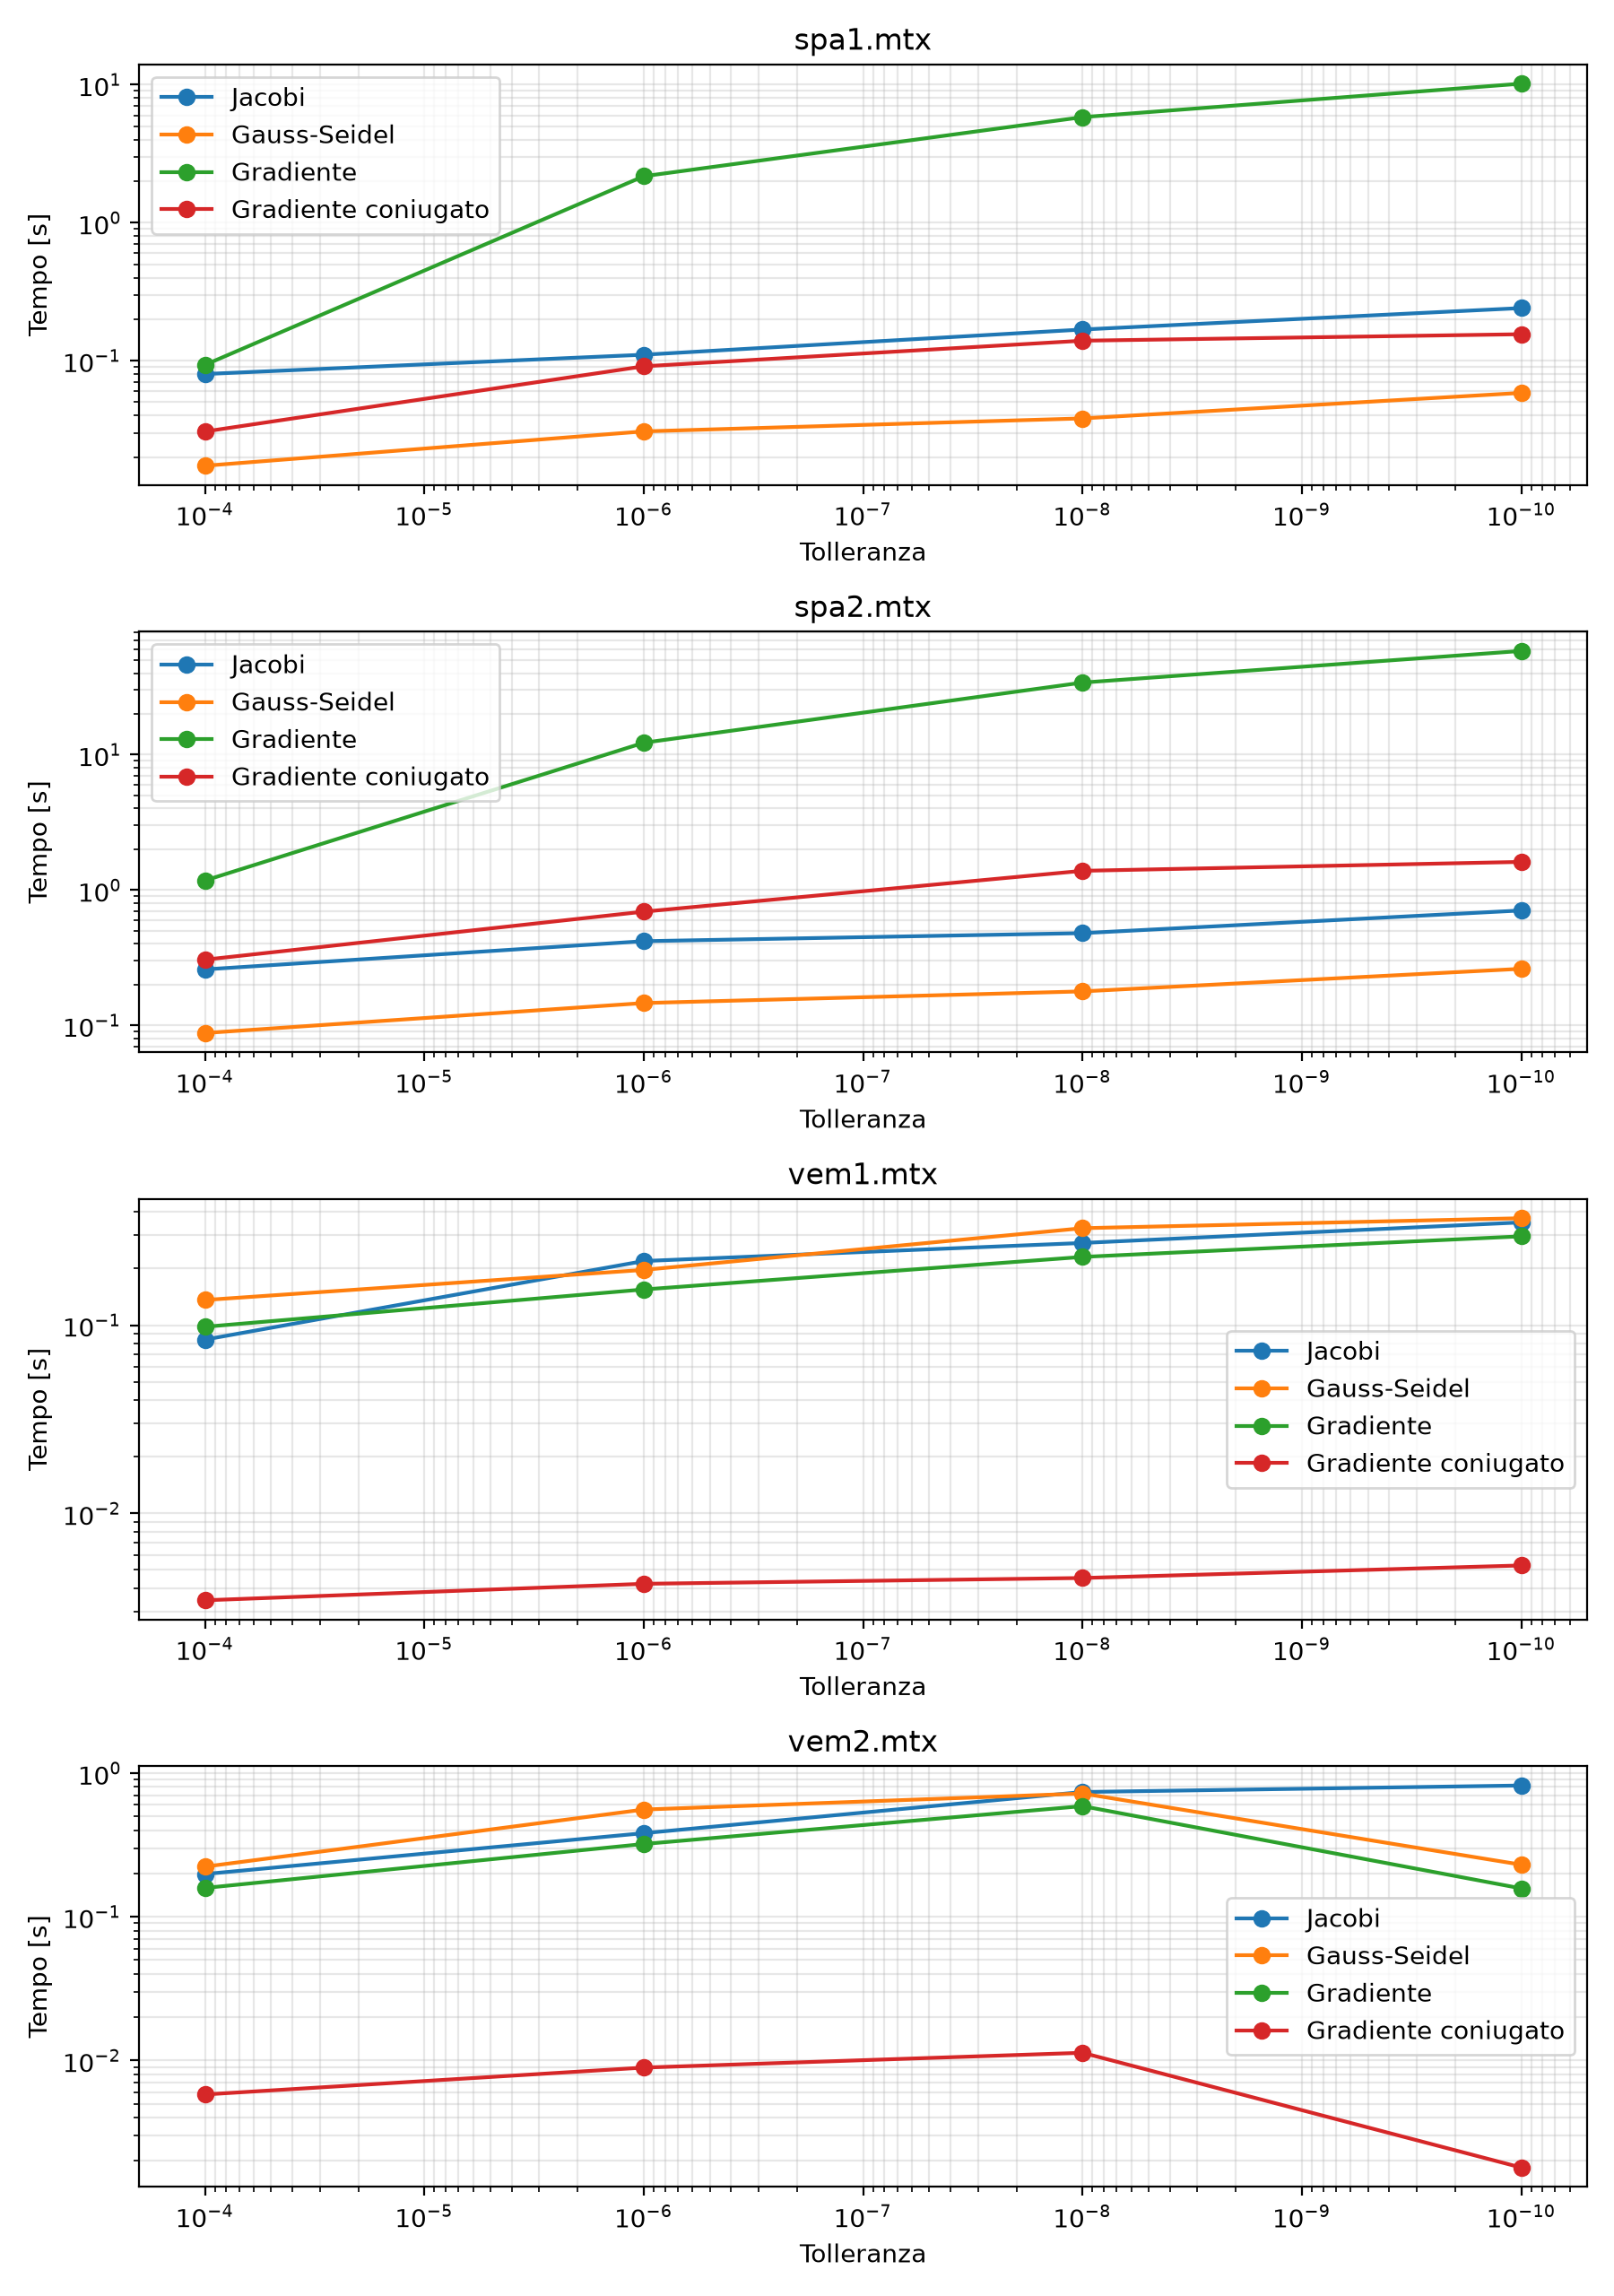
\includegraphics[width=0.85\textwidth]{results/plots/time.png}
\caption{Tempo di calcolo al variare di \texttt{tol} (scala logaritmica).}
\end{figure}

\clearpage
\subsection{Discussione comparativa}
I dati numerici e i grafici restituiscono un quadro coerente con la teoria della
PARTE 1. Riassumiamo le osservazioni principali.

\paragraph{Gauss--Seidel $\approx$ metà delle iterazioni di Jacobi.}
È esattamente quanto previsto: riusando immediatamente le componenti appena
calcolate, Gauss--Seidel fa più ``lavoro utile'' per iterazione. Ad esempio su
\texttt{vem2} a $\texttt{tol}=10^{-8}$ Jacobi richiede 5425 iterazioni contro le
2714 di Gauss--Seidel (rapporto $\approx2.0$). Il singolo passo di Gauss--Seidel
è però un po' più costoso (sweep sequenziale), perciò sulle matrici molto sparse
\texttt{vem} i tempi totali dei due metodi si equivalgono, mentre sulle
\texttt{spa} (dove Gauss--Seidel converge in pochissime iterazioni) è nettamente
il più rapido.

\paragraph{Due ``regimi'' opposti tra le famiglie di matrici.}
I metodi stazionari e quelli del gradiente rispondono a proprietà diverse della
matrice:
\begin{itemize}[leftmargin=1.6em]
  \item su \textbf{spa1/spa2} Jacobi e Gauss--Seidel sono fulminei (5--313
  iterazioni), mentre il Gradiente è lentissimo (fino a $\sim$12\,900
  iterazioni). Le \texttt{spa} sono fortemente \emph{dominanti diagonali}
  $\Rightarrow$ raggio spettrale della matrice di iterazione piccolo
  $\Rightarrow$ metodi stazionari rapidi; ma hanno $\mathrm{cond}(A)\approx
  2\cdot10^3$, e la velocità del Gradiente dipende proprio da $\mathrm{cond}(A)$,
  da cui la lentezza;
  \item su \textbf{vem1/vem2} la situazione si riequilibra: la minore dominanza
  diagonale rende Jacobi/Gauss--Seidel più lenti (migliaia di iterazioni), mentre
  il minore $\mathrm{cond}(A)\approx3$--$5\cdot10^2$ rende il Gradiente
  competitivo.
\end{itemize}
Ciò conferma che la velocità di Jacobi/Gauss--Seidel è governata dalla
\textbf{dominanza diagonale} ($\rho(P^{-1}N)$), mentre quella di
Gradiente/Gradiente coniugato è governata dal \textbf{numero di
condizionamento}.

\paragraph{Il Gradiente coniugato è il metodo più robusto e regolare.}
Converge sempre in \textbf{poche decine di iterazioni} (38--240),
indipendentemente dalla matrice, con crescita lentissima al ridursi di
\texttt{tol}. Il numero di iterazioni scala come $\sqrt{\mathrm{cond}(A)}$
(coerentemente, \texttt{spa1} con $\mathrm{cond}\approx2\cdot10^3$ richiede più
passi di \texttt{vem1} con $\mathrm{cond}\approx3\cdot10^2$) e resta sempre ben al
di sotto del limite teorico di $n$ iterazioni. È il vincitore netto sulle matrici
mal condizionate \texttt{vem}.

\paragraph{Residuo piccolo $\neq$ errore piccolo.}
A parità di \texttt{tol}, l'errore relativo sulla soluzione \textbf{non} è uguale
fra i metodi e, per quelli stazionari, vale circa $\texttt{tol}\times\text{cost}$,
con cost legato al condizionamento (relazione
$\text{errore}\lesssim\mathrm{cond}(A)\cdot\text{residuo}$). Ad esempio a
$\texttt{tol}=10^{-6}$: su \texttt{vem2} l'errore è $\sim5\cdot10^{-5}$ (circa
50$\times$ il residuo); su \texttt{spa1} il Gradiente ha errore
$\sim10^{-3}$ (circa 1000$\times$ il residuo). Il Gradiente coniugato raggiunge
invece errori molto più piccoli (fino a $\sim10^{-11}$), perché tende a ridurre
simultaneamente tutte le componenti spettrali dell'errore.

\paragraph{Tempi di calcolo.}
In secondi assoluti il quadro dipende dalla densità della matrice:
\begin{itemize}[leftmargin=1.6em]
  \item sulle \texttt{spa} (dense) il prodotto matrice--vettore è caro, quindi il
  Gradiente, che fa molte iterazioni, arriva a oltre 50\,s (\texttt{spa2} a
  $10^{-10}$), mentre Gauss--Seidel resta sotto 0.3\,s e CG sotto 1.7\,s;
  \item sulle \texttt{vem} (molto sparse) tutti i metodi sono rapidi ($<1$\,s); CG
  è comunque il più veloce in assoluto ($\le0.011$\,s) grazie al bassissimo
  numero di iterazioni.
\end{itemize}

In sintesi, su queste matrici il \textbf{Gradiente coniugato è la scelta migliore
in ogni scenario}; tra i metodi stazionari, Gauss--Seidel domina Jacobi; il
Gradiente semplice è penalizzato quando la matrice è mal condizionata (effetto
``zig-zag'').

% ==================================================================
\section{Documentazione del codice}
% ==================================================================
Il codice è documentato in modo sistematico: ogni modulo ha una docstring di
intestazione che ne descrive lo scopo, e ogni classe o funzione pubblica ha una
docstring che ne specifica comportamento, argomenti, valore di ritorno ed
eccezioni sollevate. Di seguito si riporta la documentazione modulo per modulo.

\subsection{Modulo \texttt{solvers.py}}
È il cuore della libreria: contiene i quattro metodi e lo scheletro comune.

\noindent\textbf{\texttt{SolverResult}} (dataclass). Raccoglie l'esito di una
risoluzione: \texttt{method} (nome del metodo), \texttt{x} (soluzione
approssimata), \texttt{iterations}, \texttt{elapsed} (tempo in secondi),
\texttt{residual\_relative} (residuo scalato finale), \texttt{converged}.

\noindent\textbf{\texttt{\_Iteration}} (interfaccia astratta). Incapsula lo stato
di un metodo per un singolo problema. Espone due metodi astratti:
\texttt{residual\_norm()} (norma euclidea del residuo corrente) e \texttt{step()}
(aggiornamento $\mathbf{x}^{(k)}\to\mathbf{x}^{(k+1)}$ in place).

\noindent\textbf{\texttt{IterativeSolver}} (classe base astratta). Implementa lo
scheletro comune.
\begin{itemize}[leftmargin=1.6em]
  \item \texttt{solve(A, b, tol, max\_iter=None)}: risolve $A\mathbf{x}=\mathbf{b}$
  da $\mathbf{x}^{(0)}=\mathbf{0}$, arrestandosi sul residuo scalato o al
  superamento di \texttt{max\_iter}. \emph{Output}: \texttt{SolverResult}.
  \emph{Eccezioni}: \texttt{ValueError} se la matrice non è quadrata o ha
  diagonale nulla.
  \item \texttt{\_make\_iteration(A, b, x)}: metodo astratto che costruisce
  l'oggetto iterazione specifico del metodo.
\end{itemize}

\noindent\textbf{\texttt{Jacobi} / \texttt{GaussSeidel} / \texttt{Gradient} /
\texttt{ConjugateGradient}}. Le quattro classi concrete; ciascuna fornisce solo la
propria regola di aggiornamento tramite la rispettiva classe \texttt{\_Iteration}
($P=D$ per Jacobi; $P=D+L$ con sweep per Gauss--Seidel; passo ottimo lungo
$\mathbf{r}$ per il Gradiente; direzioni $A$-coniugate per CG).

\noindent\textbf{\texttt{\_gauss\_seidel\_sweep(indptr, indices, data, diag, b,
x)}} (compilata con \texttt{@njit}). Esegue una sweep di Gauss--Seidel
aggiornando \texttt{x} in place (sostituzione in avanti sul formato CSR).

\noindent\textbf{\texttt{warmup()}}. Forza la compilazione JIT su un problema
$3\times3$, da chiamare prima delle misure di tempo.

\noindent\textbf{\texttt{\_validate\_for\_iteration(A)} / \texttt{\_safe\_norm(x)}}.
Funzioni di servizio: la prima controlla che $A$ sia quadrata e con diagonale non
nulla; la seconda restituisce la norma di un vettore, evitando la divisione per
zero quando $\mathbf{b}=\mathbf{0}$.

\subsection{Modulo \texttt{run\_assignment.py}}
Eseguibile da riga di comando per la validazione.
\begin{itemize}[leftmargin=1.6em]
  \item \texttt{main()}: parsa gli argomenti, esegue il \texttt{warmup()}, e per
  ogni matrice e tolleranza risolve con i metodi selezionati, calcola l'errore
  relativo e accumula le righe del CSV; salvo \texttt{-{}-no-plots} genera anche i
  grafici.
  \item \texttt{parse\_args()}: definisce la CLI (\texttt{-{}-matrix},
  \texttt{-{}-tol}, \texttt{-{}-method}, \texttt{-{}-max-iter},
  \texttt{-{}-output}, \texttt{-{}-no-plots}, i primi tre ripetibili).
  \item \texttt{\_resolve\_matrices} / \texttt{\_select\_solvers}: risolvono
  rispettivamente l'elenco dei file \texttt{.mtx} (tutta la cartella \texttt{dati}
  se non specificato) e il sottoinsieme di metodi da usare.
  \item \texttt{\_write\_csv(rows, path)}: serializza tutte le metriche
  (matrice, $n$, nnz, tol, metodo, errore relativo, residuo, iterazioni, tempo,
  convergenza) in \texttt{results/results.csv}.
\end{itemize}

\subsection{Moduli \texttt{plot\_results.py} e \texttt{analyze\_cond.py}}
\noindent\textbf{\texttt{plot\_results.py}}. \texttt{create\_plots(rows,
output\_dir)} produce i tre grafici (errore relativo, iterazioni, tempo); la
funzione ausiliaria \texttt{\_plot\_metric} disegna una metrica raggruppando per
matrice e metodo, con l'asse \texttt{tol} in scala logaritmica e invertito.

\noindent\textbf{\texttt{analyze\_cond.py}}. Script a margine (non parte dei
solutori): stima $\lambda_{\min}$, $\lambda_{\max}$ e $\mathrm{cond}(A)$ per ogni
matrice tramite \texttt{scipy.sparse.linalg.eigsh}, ai soli fini dei commenti
della relazione.

\subsection{Modulo \texttt{test\_assignment.py}}
Test automatici: \texttt{test\_scipy\_reads\_matrix\_market} (parser
MatrixMarket), \texttt{test\_solvers\_on\_tridiagonal\_spd} (convergenza dei
quattro metodi su una tridiagonale SPD) e
\texttt{test\_conjugate\_gradient\_is\_fast\_on\_small\_matrix} (CG converge in al
più $n$ iterazioni su un sistema piccolo).

% ==================================================================
\appendix
\section{Codice sorgente}
% ==================================================================
Di seguito si riporta il codice sorgente completo dei moduli del progetto. La
documentazione modulo per modulo è descritta nella Sezione~5.

\subsection{\texttt{solvers.py}}
\lstinputlisting[style=pyfull]{solvers.py}

\subsection{\texttt{run\_assignment.py}}
\lstinputlisting[style=pyfull]{run_assignment.py}

\subsection{\texttt{plot\_results.py}}
\lstinputlisting[style=pyfull]{plot_results.py}

\subsection{\texttt{analyze\_cond.py}}
\lstinputlisting[style=pyfull]{analyze_cond.py}

\subsection{\texttt{test\_assignment.py}}
\lstinputlisting[style=pyfull]{test_assignment.py}

\end{document}
